\documentclass[../thesis.tex]{subfiles}
\begin{document}
\chapter{Methodology}\label{cap:methodology}
This chapter introduces the main contributions of the thesis, first describing the components that constitute the solution, common to all implementations. Since the final objective of this work is to evaluate three different web crawler implementations and to understand whether it is appropriate to use the serverless paradigm in this use case, the chapter is divided into two main sections:

\begin{itemize}
    \item \autoref{sec:system_architecture} describes the main components common to all implementations, it analyses the operations performed by each component and illustrates the technology stack of our applications;
    \item \autoref{sec:implementations} comprises three subsections, each of which aims to describe in depth the underlying infrastructure of each implementation; in addition, the changes made to the code bases are explained.
\end{itemize}

\section{System Architecture}\label{sec:system_architecture}
As mentioned earlier, it is necessary to describe the architecture used at a high level, which underlies the three web crawling applications, in order to understand how the framework works. \autoref{fig:system_architecture_general} illustrates the essential modules and the two types of memorization used to store search information and \acrshort{HTML} documents.

\begin{figure}[H]
    \centering
    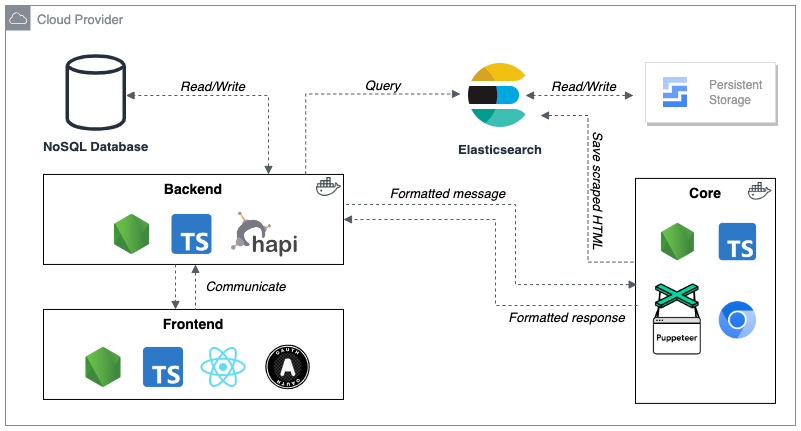
\includegraphics[width=1\textwidth]{methodology/system_architecture_general.png}
    \caption[High-level web crawlers architecture]{High-level architecture common to all web crawler implementations. Each component is shown, and the technology stack used is specified for our modules.}
    \label{fig:system_architecture_general}
\end{figure}

The frontend module provides a \acrshort{UI} for users to interact with. It incorporates \acrfull{OAuth 2.0} to ensure secure access to the platform and allows logged-in users to perform actions such as creating, analysing and deleting crawl searches. In order to start the web crawling process, users must provide a seed \acrshort{URL} for the specific site they wish to explore, specify the number of pages to crawl, name the search with a brief description, and decide whether to use browser automation or \acrshort{HTTP} requests.

The backend makes sure that the data entered are valid before creating a new document inherent to the search within the NoSQL database. It also initiates the search by forwarding the seed \acrshort{URL} and a unique identifier to the core module.

The latter loads the web page according to the chosen method, scrapes all the links in it, filters and validates them, and extracts the \acrshort{HTML} body to load the document into the Elasticsearch index. As a response, it sends the filtered links in batch to the backend, which is responsible for continuing the search or stopping it, based on the current number of visited \acrshort{URL}s that is tracked in the database.

\subsection{Indexing}
One key aspect of this application is the ability to index the \acrshort{HTML} body of visited web pages, so as to enable keyword searching. In order to create a high-availability cluster suitable for production, the smallest possible configuration comprising two nodes with a tiebreaker was chosen \cite{site:elasticsearch_cluster_conf}: a particular node that resolves deadlocks or ties when decisions require a majority vote in \gls{quorum_based_system}. As explained in \ref{sec:elasticsearch}, it was decided to deploy the \acrshort{ECK} operator to enable easy installation of the Elasticsearch module. \autoref{fig:architecture_elasticsearch} illustrates some of the resources required for proper operation.

\begin{figure}[H]
    \centering
    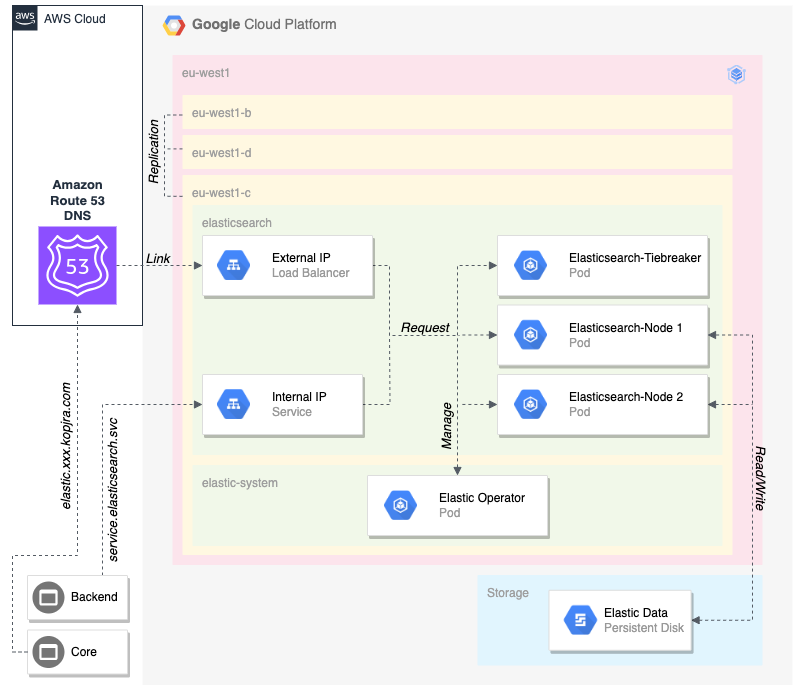
\includegraphics[width=1\textwidth]{methodology/architecture_elasticsearch.png}
    \caption[Elasticsearch cluster configuration]{The smallest possible Elasticsearch cluster configuration that is suitable for production deployments. It ensures high availability and resiliency to the failure of an individual node.}
    \label{fig:architecture_elasticsearch}
\end{figure}

The three \gls{pod}s inside the elasticsearch \gls{ns} compose the cluster\footnote{Any time that you start an instance of Elasticsearch, you are starting a node. A collection of connected nodes is called a cluster. See \href{https://www.elastic.co/guide/en/elasticsearch/reference/current/modules-node.html}{https://www.elastic.co/guide/en/elasticsearch/reference/current/modules-node.html} for more details.}, each node has one or more roles to play during the execution, in particular:

\begin{itemize}
    \item \textit{Node 1} and \textit{Node 2} have \texttt{master} and \texttt{data} roles, they interact directly with the persistent storage to index and query the uploaded documents. Since Elasticsearch is a \gls{quorum_based_system}, it is necessary for there to be multiple \texttt{master} or \texttt{voting\_only} nodes within the cluster;
    \item \textit{Tiebreaker}, has only \texttt{master} and \texttt{voting\_only} roles, it is necessary to perform election also with one node failure and it doesn't interact with the persistent storage. It intervenes when the leading nodes are evenly divided or cannot reach a consensus due to network problems.
\end{itemize}

The installation includes an internal \gls{svc} by default, and with a simple change to the configuration \acrshort{YAML} file, an external \gls{svc} can be added. The latter exposes a virtual \acrshort{IP} address that was linked to a \acrshort{DNS} name through Amazon \gls{route_53}. In both internal and external connections, the Elasticsearch module requires \acrshort{API} token authentication.

Once the deployment is done, it is possible to create a new index that will store the scraped \acrshort{HTML} body of the visited web pages. Thanks to the text analysis process, Elasticsearch provide a simple way of converting unstructured text into a structured format that is optimized for search. In our case, the documents indexed by the platform include three fields: \texttt{crawl\_search\_id}, \texttt{url} and \texttt{html}. The first is necessary to understand what search that page refers to; the others contain actual information about the web page. During the ingestion or search phase, tokenization and normalization are essential, together with the analyzer package, they define the rules to perform a full-text search. Specifically, the two custom analyzers \texttt{html\_analyzer} and \texttt{html\_search} were defined, which perform respectively the following operations:

\begin{enumerate}
    \item strips \acrshort{HTML} elements, removes punctuation and white spaces, casts all to lowercase, converts outlier characters to their \acrshort{ASCII} equivalent when possible and removes stop words of different alphabets (ingestion phase);
    \item the same above, without the strip of \acrshort{HTML} elements (search phase).
\end{enumerate}

Once the index is populated, it will be possible to search one or more keywords: the response will show all \acrshort{URL}s that in the \texttt{html} field contain those words or, depending on the parameters chosen in the query, at least one of them.

\subsection{Core}
The core module is the beating heart of the application. It receives messages from the backend and starts the web crawling process, which is divided into several stages. Both implementations that exploit the serverless paradigm operate following this workflow; on the other hand, the microservices variant will be analyzed separately in \autoref{subsec:krawler-pod}.

An example of an initial message is shown in \autoref{code:request_msg_core}, you can specify an optional fourth field within the \acrshort{JSON} object called \texttt{credentials}, which is needed in case you have to perform automatic login to the site you want to crawl (n.b. it is a limited feature, working only in certain types of sites that contain standard authentication forms). \autoref{fig:workflow_core} illustrates all the intermediate steps of a search, according to the method chosen by the user.

\begin{lstlisting}[language=json, captionpos=b, caption={[Sample initial message for the core]Example of an initial message received by the core module.}, label={code:request_msg_core}]
[
   {
      "id":"65d5f46d7a848e6e8bf41bb3",
      "url":"https://tg24.sky.it/",
      "browserAutomation":"true"
   }
]
\end{lstlisting}

\begin{figure}[H]
    \centering
    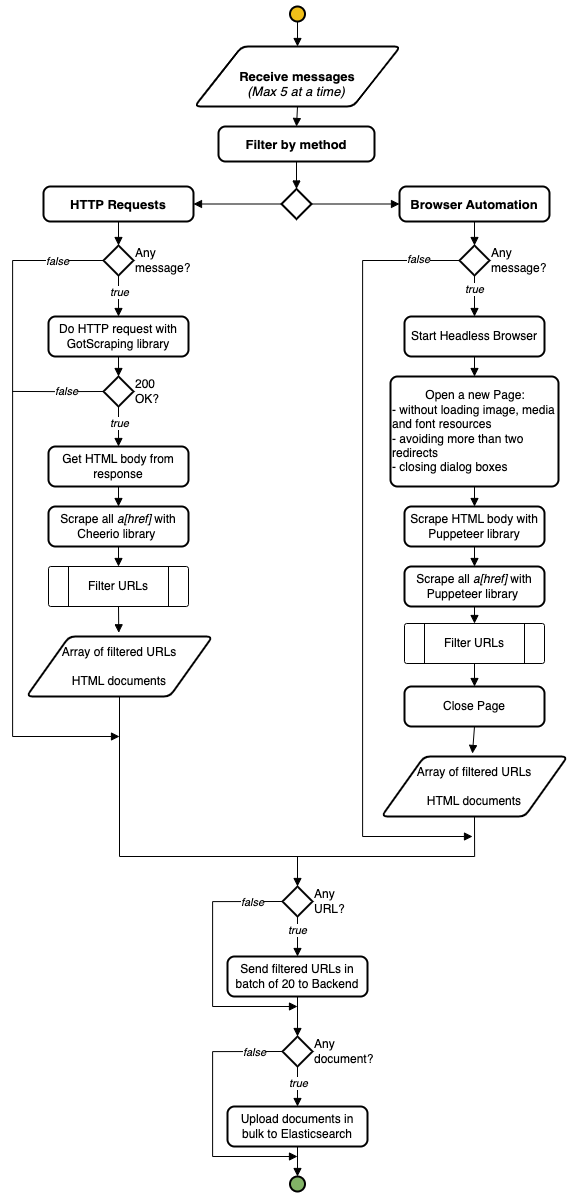
\includegraphics[width=.73\textwidth]{methodology/workflow_core.png}
    \caption[Core module workflow]{Diagram describing the operations performed by the core module, in the two serverless implementations.}
    \label{fig:workflow_core}
\end{figure}

Functions can process a maximum of 5 messages at a time. After receiving an array in input, it is filtered to separate messages according to the \texttt{browserAutomation} field. The differences between the two methods will now be analyzed.

\texttt{HTTP request} For each message inside the filtered array with the \texttt{browserAutomation} field equal to \textit{false}, get the \texttt{url} field and perform an \acrshort{HTTP} request using the \gls{got_scraping} library \cite{site:got_scraping}. If the response status code is \textit{200 OK}, retrieve the \acrshort{HTML} body of the web page and scrape all the \textit{a[href]} selectors using \gls{cheerio} library \cite{site:cheerio}. Once the \textit{href} attributes have been extracted from the \textit{a} selectors and a set is created with them, the process of filtering \acrshort{URL}s is carried out.

\texttt{Browser automation} If there is any message inside the filtered array with the \texttt{browserAutomation} field equal to \textit{true}, start the Chromium browser in headless mode, get the \texttt{url} field and open a new tab (n.b. Puppeteer calls it page) for each of them. In these new tabs, the request interceptor is enabled so that image, media and font resources are not loaded and redirects do not exceed two-hop limits. Also, if dialog boxes are present, they are closed. When the \gls{domcontentloaded} event is fired, it is possible to retrieve the \acrshort{HTML} body of the web page and scrape all the \textit{a[href]} selectors using directly Puppeteer. Once the \textit{href} attributes have been extracted from the \textit{a} selectors and a set is created with them, the same \acrshort{URL} filtering process used in the previous method and illustrated in \autoref{fig:workflow_core_filter} is performed.

\begin{figure}[H]
    \centering
    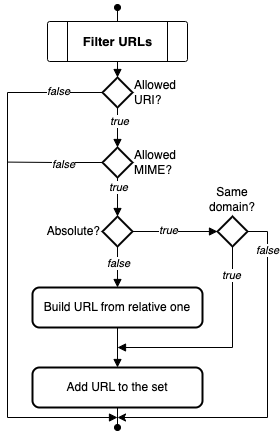
\includegraphics[width=.4\textwidth]{methodology/workflow_core_filter.png}
    \caption[Filter \acrshort{URL}s process workflow]{Diagram describing the steps performed to filter \acrshort{URL}s.}
    \label{fig:workflow_core_filter}
\end{figure}

Given the array containing all the raw links, it is necessary to filter them as follows:

\begin{enumerate}
    \item Check the type of \acrshort{URI}, discarding those not of interest with a regex (e.g. \textit{mailto},\textit{tel}, \textit{javascript}, etc.);
    \item Check the \acrshort{MIME} resource type according to the allowed types (e.g. \textit{text}, \textit{html}, \textit{application/x-httpd-php} etc.);
    \item If both conditions are met, check whether the \acrshort{URL} is absolute or relative. In the first case, it will be sufficient to verify that the host of the seed \acrshort{URL} is contained therein; in the latter, it is necessary to reconstruct the absolute \acrshort{URL};
    \item The filtered \acrshort{URL} can be added to the set, which will then be output by the function in the form of an array.
\end{enumerate}

Finally, the filtered \acrshort{URL}s inside the array are sent to the backend in batches of 20 as shown in \autoref{code:response_msg_core} and the \acrshort{HTML} documents are uploaded in bulk to the Elasticsearch index along with the source \texttt{url} and the \texttt{id} to link the search.

\begin{lstlisting}[language=json, captionpos=b, caption={[Sample of core response message]Example of a response message sent by the core.}, label={code:response_msg_core}]
{
   "id":"65d5f46d7a848e6e8bf41bb3",
   "batch":[
      "https://tg24.sky.it/edizioni-locali",
      "https://tg24.sky.it/salute-e-benessere/alimentazione",
      etc.
   ]
}
\end{lstlisting}

With these two search methods available, we offer users the flexibility to choose according to their needs, allowing each person to decide which method to use: more realistic browsing that takes advantage of browser automation and loads the \acrshort{DOM} of each web page, or using \acrshort{HTTP} requests that are certainly faster but with possible limitations imposed by web site administrators.

\subsection{Backend}
The backend module is needed to manage the creation, interaction, and deletion of searches and, in particular, allows the web crawling process to continue once it has started. It was developed according to the principles of \gls{hex_arch}, taking advantage of a scaffolder used in Kopjra as a basic project structure generator.

It connects to a MongoDB \gls{no_sql} and interacts with three collections defined as follows:

\begin{itemize}
    \item \texttt{crawlsearches}, where all the information about searches is stored, it is necessary to keep track of the crawling status and the number of \acrshort{URL}s visited so far, two useful timestamps related to creation and last update are also tracked. Some important fields in this collection are \textit{seed}, \textit{visitedUrls}, \textit{maxVisitedUrls}, and \textit{status};
    \item \texttt{results}, stores all \acrshort{URL}s obtained through the core module and keeps track of those visited; a timestamp related to the creation is also tracked. Some important fields in this collection are \textit{url}, \textit{visited}, and \textit{crawlSearchId};
    \item \texttt{users}, manages all stuff related to the user, such as credentials, \acrshort{OAuth 2.0} token, etc. It is fundamental during the authentication stage.
\end{itemize}

As a backend application, it offers all \acrshort{CRUD} operations on the first two collections. Still, we will focus mainly on the paths of interest that manage the flow of creating a search up to its completion and allow you to search in the results obtained.

\texttt{POST /crawls} \autoref{code:post_crawls} shows an example of a valid payload to use on this route. Once the body has been validated, an object within the \texttt{crawlsearches} and \texttt{results} collections is created, where the \textit{visited} field is set to true for the \textit{seed} \acrshort{URL}. Based on the implementation, a first message is sent to the core module through \acrshort{SQS} or \gls{rabbit_mq} broker.

\begin{lstlisting}[language=json, captionpos=b, caption={[Sample of new search creation payload]Example of a valid payload message to create a new search.}, label={code:post_crawls}]
{
   "seed":"https://tg24.sky.it/",
   "name":"tg24 sky news",
   "maxVisitedUrls":100,
   "browserAutomation":true
}
\end{lstlisting}

\texttt{POST /internal/results} The same payload illustrated in \autoref{code:response_msg_core} is used on this route. When the core module starts sending data, the data does not go directly to the backend; instead, \acrshort{SNS} or \gls{rabbit_mq} is exploited, depending on the implementation. Once the message is forwarded by one of the previous technologies and received by the backend, it creates many objects inside the \texttt{results} collection based on the number of \acrshort{URL}s in the \textit{batch} field, setting them all to unvisited. Now, the current crawl search identified by the \textit{id} can continue or not, there may be several scenarios:

\begin{itemize}
    \item the search has already reached the finished \textit{status} due to previous calls on the same internal route;
    \item the search has not yet reached the finished \textit{status}, so the backend needs to check if the current number of \textit{visitedUrls} has not exceeded the \textit{maxVisitedUrls}. If this condition is verified, it increments the number of \textit{visitedUrls}, retrieves a new unvisited \acrshort{URL} from the \texttt{results} collection and sends it to \acrshort{SQS};
    \item the search has not yet reached the finished \textit{status} but the current number of \textit{visitedUrls} has reached the \textit{maxVisitedUrls} value, so the search \textit{status} is updated to finished;
    \item the search has not yet reached the finished \textit{status} nor the \textit{maxVisitedUrls} value, but there are no more visitable \acrshort{URL}s within the \texttt{results} collection, so the search \textit{status} is updated to finished.
\end{itemize}

\texttt{GET /crawls/{crawlSearchId}/results} During the crawling process, as we already said, the \acrshort{HTML} body of each visited \acrshort{URL} is indexed. This route allows keyword searches within the \acrshort{URL} string and inside the index managed by Elasticsearch, which contains the \acrshort{HTML} body of the web pages visited. Just specify the \textit{url} parameter for the first type of search, and the \textit{htmlQuery} and \textit{strictHtmlQuery} parameters for the second. In particular, \textit{strictHtmlQuery} is a boolean that specifies whether the keywords must all be present in the document or at least one is sufficient.

Having explained the backend's role in creating and completing a search as well as keyword searching in the results, let us now turn to its architecture, illustrated in \autoref{fig:architecture_backend}.

\begin{figure}[H]
    \centering
    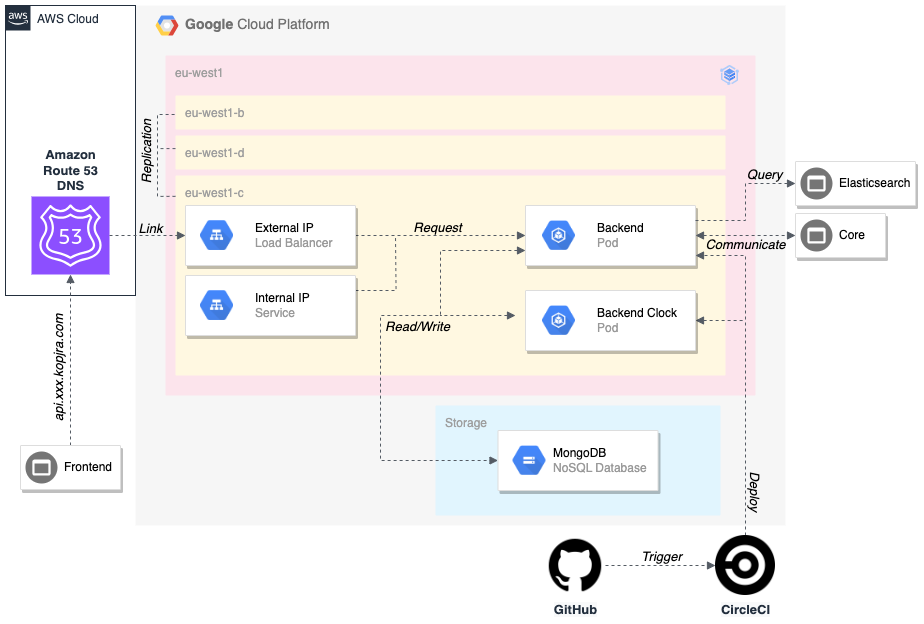
\includegraphics[width=1\textwidth]{methodology/architecture_backend.png}
    \caption[Backend architecture]{Backend architecture.}
    \label{fig:architecture_backend}
\end{figure}

\gls{docker} was used to define a multi-stage build, which, together with a \texttt{node:alpine} base image, allowed us to optimize our \gls{container}. The \gls{circle_ci} tool builds and pushes the \gls{docker} image, and then leverages the \gls{kustomize} configuration files to deploy in a standard way our backend application on \acrfull{GKE}. Several resources have been defined in the \gls{k8s} files, such as \gls{config_map}, \gls{secret}, \gls{deployment}, \gls{svc} and \gls{ingress}. The latter manages the external access to the backend so that the frontend can query it directly from the \acrshort{DNS} name specified in Amazon \gls{route_53} service.

A note on why a clock \gls{pod} was also deployed: it checks every 10 minutes if, for some reason, a search crashes and does not reach the finished state, updating it to a general error state if the last change was within 5 minutes.

\subsection{Frontend}
The frontend module makes life easier for users who want to use this application. It is a \acrshort{SPA} written in React and deployed inside an \acrshort{S3} bucket, according to \cite{site:deploy_react_s3}. Again, a scaffolder provided by Kopjra was used to create a base project structure and start the development.

The architecture is illustrated in \autoref{fig:architecture_frontend}, mainly leveraging \acrshort{AWS} services such as \acrshort{S3}, \gls{cloudfront}, \acrshort{ACM} and \gls{route_53}. In addition, the deployment is performed using \gls{circle_ci}'s \texttt{aws-s3} orb\footnote{See \href{https://circleci.com/developer/orbs/orb/circleci/aws-s3}{https://circleci.com/developer/orbs/orb/circleci/aws-s3} for more details.}, which allows us to synchronize and copy all files inside our repository to an \acrshort{S3} bucket.

\begin{figure}[H]
    \centering
    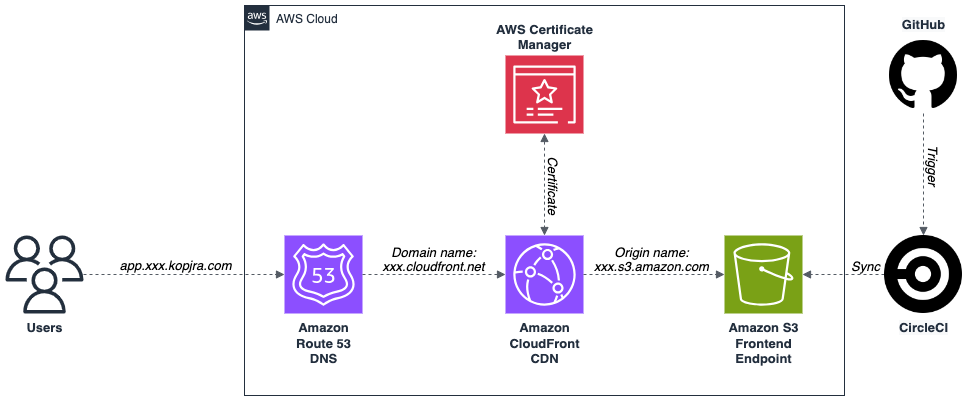
\includegraphics[width=1\textwidth]{methodology/architecture_frontend.png}
    \caption[Frontend architecture]{Frontend architecture.}
    \label{fig:architecture_frontend}
\end{figure}

The ability to authenticate with your Google account by leveraging \acrshort{OAuth 2.0} is given, so one does not have to create an additional user account.

Some screenshots are given in \autoref{appendix:screenshot} so that the various scenarios can be better understood.

\section{Implementations}\label{sec:implementations}
The various modules that make up the web crawling application were described so as to get an overview of the behaviour of each of them. In this section, we want to take an in-depth look at the three proposed implementations, dwelling on the configuration of the core module of each. Similar architectures to the previous ones will then be shown, with some variations highlighted in orange.

\subsection{\texttt{krawler} on AWS Lambda}
In this scenario, the core module is deployed in a Lambda function, and the I/O communications are managed by \acrshort{SQS} and \acrshort{SNS} services respectively. The first challenge was to install a browser inside the latest NodeJS image\footnote{See \href{https://gallery.ecr.aws/lambda/nodejs}{https://gallery.ecr.aws/lambda/nodejs} for more details.} provided by \acrshort{AWS}. One simple method would be installing Google Chrome directly, as explained in \cite{site:universal_chrome}, but unfortunately, it significantly enlarges image size. Using \texttt{chrome-aws-lambda} \cite{site:chrome_aws_lambda} could have been an option thanks to the small size of the binary and the updates made a few days after Puppeteer's, but it is no longer maintained. The solution chosen involves the use of a fork of the latter, called \texttt{chromium} \cite{site:chromium_aws_lambda}, which is no longer tied directly to Puppeteer but works perfectly with it and weighs a few megabytes more. It was then installed as a dependency along with \texttt{puppeteer-core}, without additional instructions within the \gls{dockerfile}. Again, a multi-stage build was defined to optimize our \gls{container}. \autoref{fig:architecture_krawler_aws} illustrates the specific architecture of this implementation.

\begin{figure}[H]
    \centering
    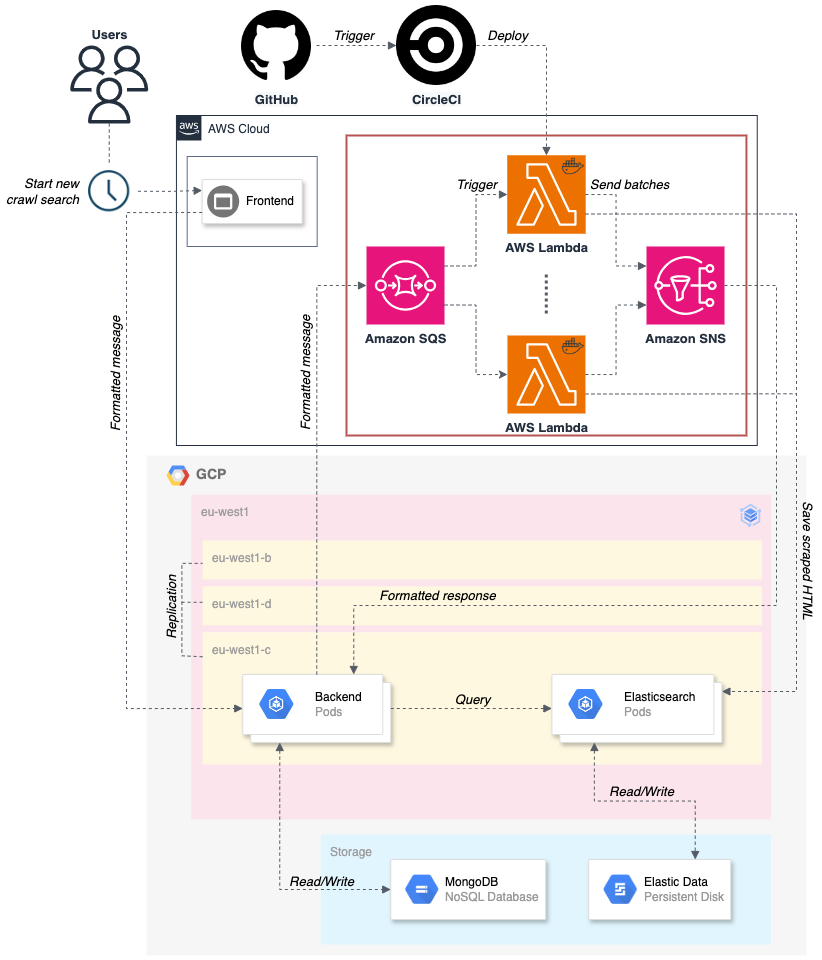
\includegraphics[width=1\textwidth]{methodology/architecture_krawler_aws.png}
    \caption[AWS implementation]{Application on AWS.}
    \label{fig:architecture_krawler_aws}
\end{figure}

The deployment was managed by \gls{circle_ci}, which handles the image building process, pushes the \gls{container} image into a registry, and uses the \acrshort{AWS} \acrshort{CLI} to update the Lambda function, previously configured with 1280MB of memory and 60s of timeout. It is not possible to explicitly state the computational capacity because it varies according to the allocated memory (1769MB of memory has the equivalent of one vCPU \cite{site:lambda_memory_cpu}) and the timeout was useful in case some web pages took too long to load.

\acrshort{SQS} is used as a trigger for our Lambda function. Through it, we were able to choose the number of messages contained in each batch, and processed by the function at each invocation. The parameters set are described below with their corresponding value :

\begin{itemize}
    \item \textit{Batch size} defines the maximum number of messages to send to the function and was set to 5;
    \item \textit{Batch window} specifies the maximum amount of time to gather messages before invoking the function. It was set to 20 seconds;
    \item \textit{Maximum concurrency} represents the maximum number of concurrent functions that the event source can invoke. Since we had to perform a series of tests with the other implementations as well, it was decided to set it to 100.
\end{itemize}

% TODO: add or not? -> No failure destination has been configured.
During its execution, the core sends batch results to \acrshort{SNS}, which acts as a deliverer and is responsible for notifying the registered endpoint. The latter points to the \texttt{/results/internal} route of the backend, made accessible by the \acrshort{DNS} name previously registered in \gls{route_53}.

To recap, the backend module receives a new crawl search request and forwards it to \acrshort{SQS} using the specific TypeScript \acrshort{SDK}. Next, \acrshort{SQS} sends this message to Lambda which is responsible for processing them and sends batches of \acrshort{URL}s to \acrshort{SNS} and \acrshort{HTML} documents to Elasticsearch. Finally, \acrshort{SNS} forwards the backend module with the results, which may or may not continue the crawling process.

\subsection{\texttt{kn-krawler} on Knative}
In this scenario, the core module and backend have been deployed using Knative, while I/O communications are handled by a \gls{rabbit_mq} broker \cite{site:knative_rabbitmq} that is responsible for routing all the events, represented by the CloudEvents \cite{site:cloudevents} specification. The choice was made to use \gls{rabbit_mq} \cite{site:rabbitmq} instead of \gls{kafka} as the message deliverer because it is lighter and requires fewer computational resources; in addition, when this thesis work was started the integration of \gls{kafka} within the Knative Eventing ecosystem was still in beta. In this case, the browser installation was easier, the latest NodeJS Alpine image was used, and thanks to its package manager, it was possible to install Chromium from the community repository. The \texttt{faas-js-runtime} framework \cite{site:faas-js-runtime} was used to handle requests on the core module and a multi-stage build was defined to further optimize the \gls{container} image, ensuring the highest efficiency level.

Some preliminary steps to install Knative components and \gls{rabbit_mq} operator are given in \autoref{code:knative_install_script}. Then, you must deploy a \gls{rabbit_mq} cluster as defined in \autoref{code:rabbitmq_cluster}, allowing the broker we will configure in \autoref{code:rabbitmq_broker} to function properly. \autoref{fig:architecture_krawler_kn} shows the specific architecture of this implementation.

\begin{figure}[H]
    \centering
    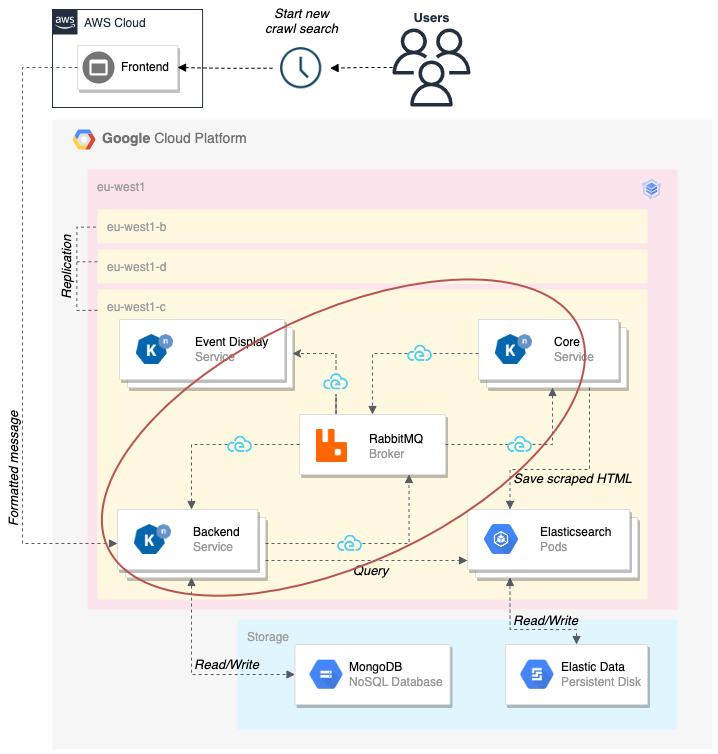
\includegraphics[width=1\textwidth]{methodology/architecture_krawler_kn.png}
    \caption[Knative implementation]{Application on Knative.}
    \label{fig:architecture_krawler_kn}
\end{figure}

You can immediately notice an additional \gls{pod} called \textit{Event Display}. It is used as a message viewer for the \acrfull{DLS} of the broker and for general logging, it scales up from zero when there is any message. Its Knative deployment is described by \autoref{code:event_display}.

The backend module was also deployed using Knative as described in \autoref{code:kn_kapturer_be}, with a minimum scale attribute equal to 1. It communicates with the broker leveraging the CloudEvents \acrshort{SDK} \cite{site:cloudevents_js} for TypeScript and receives CloudEvents on the internal route. One lacking feature, compared to the previous implementation, is the ability to specify a \textit{batch\_size}; in fact, changes were made by the backend to send, within a single CloudEvent, a list of messages of maximum length 5. An example of a message it sends is shown in \autoref{code:kn_ce_request_be}.

\begin{lstlisting}[language=json, captionpos=b, caption={[Sample of search start message from backend]Example of search start message on Knative from backend module. The mandatory fields that CloudEvents must have were not reported.}, label={code:kn_ce_request_be}]
{
   "type":"dev.kapturer.crawls",
   "source":"kn-kapturer-be",
   "datacontenttype":"application/json",
   "data":[
      {
         "id":"65d5f46d7a848e6e8bf41bb3",
         "url":"https://tg24.sky.it/",
         "browserAutomation":false
      }
   ]
}
\end{lstlisting}

The core module takes advantage of the scale-to-zero feature, enabling it to automatically terminate idle replicas that have remained inactive for a designated duration. The Knative deployment configuration for this service is detailed in \autoref{code:kn_krawler}. The various autoscaling annotations show that the metric chosen to scale up this service is concurrency, which determines the number of simultaneous requests that can be processed by each replica of an application at any given time. A cap of 100 concurrent functions has been set, which controls the maximum number of replicas that each revision should have. Knative will attempt to never have more than this number of replicas running or in the process of being created at any one point in time. Also, it is possible to specify a soft or hard limit, which represents a targeted threshold and an enforced upper bound on concurrency, respectively. The \texttt{containerConcurrency} field defines a hard limit of 1; this value defines the exact number of requests that can be sent to a replica at any time. The concurrency value can be further adjusted using the \texttt{target-utilization-percentage} attribute, which explains the percentage of the previously specified target that the autoscaler must actually achieve. In other words, it will create a new replica as soon as any concurrent request is detected. This means that the autoscaler will initiate a new replica to handle potential additional requests even with just one concurrent request.

When the \gls{rabbit_mq} broker receives an event, it then takes care of routing it according to the subscribers to that event type. Therefore, communications to the backend and core modules, occur via two triggers that filter events based on the \textit{source} and \textit{type} fields of the CloudEvent, as can be seen from their definition in \autoref{code:kn_trigger}. The \texttt{parallelism} attribute helps to define the number of workers the trigger creates to consume messages off the queue and dispatch them to the sink.

\subsection{\texttt{krawler-pod} on Kubernetes}\label{subsec:krawler-pod}
The previous implementations follow the serverless paradigm, either delivered via service from a cloud provider such as \acrshort{AWS} or managed in-house through the deployment of Knative, an open-source serverless solution. In this last implementation, we want to use the resources provided by \gls{k8s}, leveraging the microservices paradigm.

A lot of responsibilities regarding search management are taken away from the backend module. It still handles \acrshort{CRUD} operations, but it is no longer concerned with the termination of searches. As can be seen from \autoref{fig:architecture_krawler_pod}, when the backend receives a request to create a search, a new \gls{job} resource is added to the cluster. The latter creates a \gls{pod} that handles the entire search to completion, visiting the number of web pages specified by the \textit{maxVisitedUrls} field.

\begin{figure}[H]
    \centering
    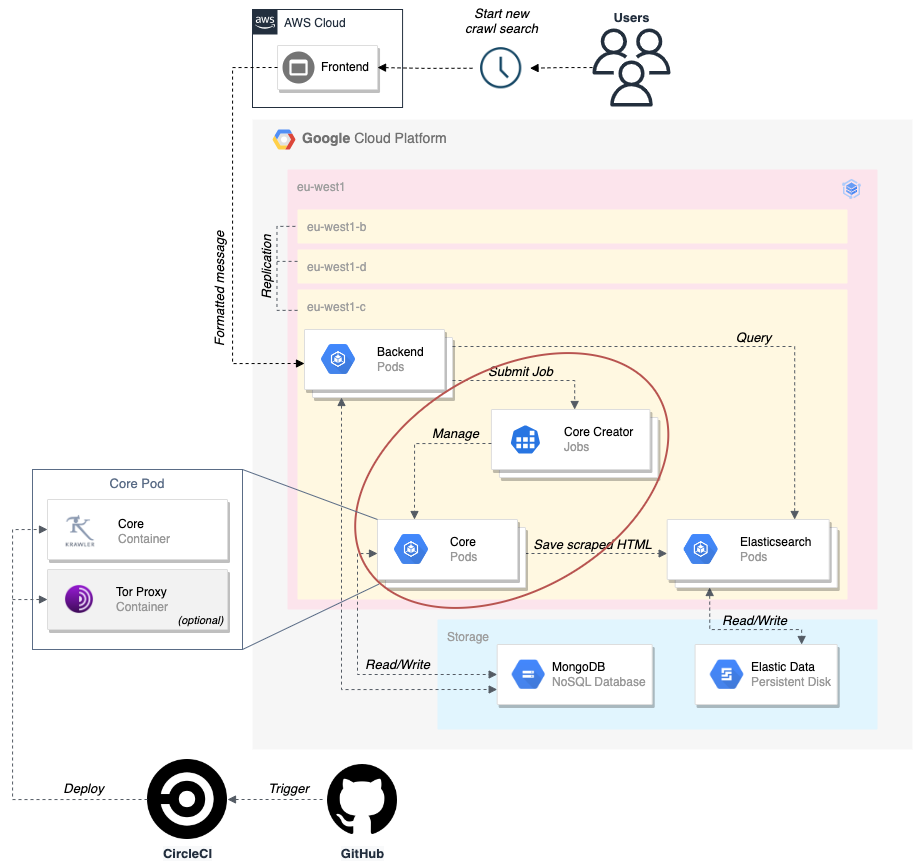
\includegraphics[width=1\textwidth]{methodology/architecture_krawler_pod.png}
    \caption[Kubernetes implementation]{Application on Kubernetes.}
    \label{fig:architecture_krawler_pod}
\end{figure}

In more detail, the backend after creating the search document within the \texttt{crawlsearch} collection, leverages the \gls{k8s} \acrshort{API} client \cite{site:k8s_client_js} to programmatically define a comprehensive set of resources, including \gls{container}, \gls{pod} and \gls{job}. These resources are encapsulated sequentially, akin to a matryoshka doll, and they compose the object that will be submitted to the cluster. The operation of submitting a \gls{job} without permission cannot be performed, which is why a \acrfull{RBAC} policy was added through the definition of \gls{svc_account}, \gls{role} and \gls{role_bind} resources.

All useful search information is passed to the core via environment variables injected into the \gls{container} so that it can handle the search autonomously since it connects directly to the database. The definition of \gls{dockerfile} is the same as that used in the Knative core, so the browser was installed the same way using \acrshort{APK}. Due to the fact that this implementation has no concurrency, it was decided to visit 10 \acrshort{URL}s at a time instead of 5 to speed up searches, slightly increasing the computational capacity and leaving the memory limit at 1280MB. In addition, thanks to the behaviour of this architecture, it was possible to add two interesting features:

\begin{enumerate}
    \item stop and resume searches that have been started but not yet finished;
    \item possibility of performing web crawling on \textit{.onion} sites when the browser automation method is chosen, thanks to the optional use of a \gls{side_car_container} that acts as a \acrshort{TOR} proxy.
\end{enumerate}

Analyzing the serverless implementations, surely stopping a search for which invocation requests have already been sent is not feasible by paradigm, since there is no storage of information and the overall status of the search is unknown. Also, injecting a \gls{side_car_container} inside a function would only slow its execution, considering the proxy tor startup time, which is on the order of a few minutes. A microservices-oriented implementation strategy involves maintaining a continuously running \gls{pod} serving as a proxy tor. In the context of Knative, individual concurrent functions can specify the \gls{pod}'s cluster domain name as proxy \acrshort{URL} to perform web crawling on \textit{.onion} websites.

Both \gls{container}'s sources have been placed for convenience in the same GitHub repository, in different folders. For each commit, the eventual build and submission image to the registry is handled by \gls{circle_ci} using \texttt{path-filtering} orb\footnote{See \href{https://circleci.com/developer/orbs/orb/circleci/path-filtering}{https://circleci.com/developer/orbs/orb/circleci/path-filtering} for more details.}. Changing even a single file within the folder will determine whether or not the pipeline will continue in that folder.

\end{document}